\documentclass{article}

\usepackage[czech, english]{babel} \usepackage[T1]{fontenc} % pouzije EC fonty
\usepackage[utf8]{inputenc}
\usepackage{gensymb}
\usepackage{amssymb,amsmath}
\usepackage{graphicx}
\usepackage{xfrac}

\setlength{\parindent}{0cm}

\begin{document}

\providecommand{\abs}[1]{\lvert#1\rvert}

\title{Backtracking - Report}
\author{Nicolas Boileau, Simon Stastny}

\maketitle

\section{Description of implementation}

We implemented algoritm solving the K-Queens puzzle with the use of backtracking
search. In our implementation the unassigned variable is selected based on size
of its domain by default: always the variable with smallest domain is selected.
This approach makes the algorithm to run significantly faster than the version
where is the unassigned variable picked based on its order in array of variables.


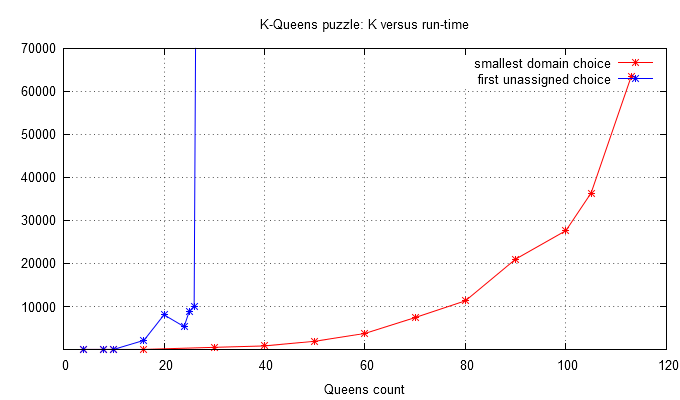
\includegraphics[width=340,height=200]{plot/queens.png}

The figure above plots performance results of both approaches. Number of
queens if shown on x-axis and run time in millisecons on y-axis. Difference between
approaches is apparent.

\newpage

\section{Solution for 8-Queens puzzle}

X \_ \_ \_ \_ \_ \_ \_ 

\_ \_ \_ \_ X \_ \_ \_ 

\_ \_ \_ \_ \_ \_ \_ X 

\_ \_ \_ \_ \_ X \_ \_ 

\_ \_ X \_ \_ \_ \_ \_ 

\_ \_ \_ \_ \_ \_ X \_ 

\_ X \_ \_ \_ \_ \_ \_ 

\_ \_ \_ X \_ \_ \_ \_ 


\section{Solution for 16-Queens puzzle}

X \_ \_ \_ \_ \_ \_ \_ \_ \_ \_ \_ \_ \_ \_ \_ 

\_ \_ X \_ \_ \_ \_ \_ \_ \_ \_ \_ \_ \_ \_ \_ 

\_ \_ \_ \_ X \_ \_ \_ \_ \_ \_ \_ \_ \_ \_ \_ 

\_ \_ \_ \_ \_ \_ \_ \_ \_ \_ \_ \_ X \_ \_ \_ 

\_ \_ \_ \_ \_ \_ \_ \_ \_ \_ X \_ \_ \_ \_ \_ 

\_ \_ \_ X \_ \_ \_ \_ \_ \_ \_ \_ \_ \_ \_ \_ 

\_ \_ \_ \_ \_ \_ \_ \_ \_ \_ \_ \_ \_ \_ X \_ 

\_ \_ \_ \_ \_ \_ X \_ \_ \_ \_ \_ \_ \_ \_ \_ 

\_ \_ \_ \_ \_ \_ \_ \_ \_ \_ \_ \_ \_ \_ \_ X 

\_ \_ \_ \_ \_ \_ \_ \_ \_ \_ \_ \_ \_ X \_ \_ 

\_ X \_ \_ \_ \_ \_ \_ \_ \_ \_ \_ \_ \_ \_ \_ 

\_ \_ \_ \_ \_ \_ \_ X \_ \_ \_ \_ \_ \_ \_ \_ 

\_ \_ \_ \_ \_ X \_ \_ \_ \_ \_ \_ \_ \_ \_ \_ 

\_ \_ \_ \_ \_ \_ \_ \_ X \_ \_ \_ \_ \_ \_ \_ 

\_ \_ \_ \_ \_ \_ \_ \_ \_ \_ \_ X \_ \_ \_ \_ 

\_ \_ \_ \_ \_ \_ \_ \_ \_ X \_ \_ \_ \_ \_ \_ 



\end{document}
